\section{Detailed Qualitative Cognitive Load Breakdown}
\label{apdx:cog_qual}

In addition to the discussion on cognitive load sources presented in the main text, we provide additional details on the six cognitive dimensions. Among all dimensions, we also provide the codes representing different types of demand in a table form. The shaded cells represent the percentage of participants citing each source of mental demand, allowing for comparison within columns. The abbreviations in the columns: ST (Short Text Interface), S2P (Short Two-phase Interface), LT (Long Text Interface), and L2P (Long Two-phase Interface). Short and Long refer to the sum across both interfaces; Text and Inter refer to the sum across both survey lengths. We include Sparklines for comparisons across these experiment groups. Future studies can use these as initial codebooks to conduct interface studiues on preference construction.

\section{Sources of Mental Demand}
\label{apdx:mental}
Mental demand refers to the amount of mental and perceptual activity required to complete a task. Table~\ref{apdx:mental_table} lists all the mental demand codes. Figure~\ref{fig:mental_cog_score} shows the boxplot of participant's subscale response.

\label{apdx:mental_table}
\begin{table}[h!]
   \caption{This table lists all the causes participants mentioned as contributing to their Mental Demand.}
   \Description{A table presenting mental demand across categories such as Budget Management (track credits, maximize usage), Preference Construction (prioritization, resource allocation), and Demand from Experiment Setup. Sparklines and percentage bars are used to visually represent the data across four interface versions (ST, S2P, LT, L2P) and experiment conditions (Short, Long, Text, Inter). The bars show higher mental demand in areas like Budget Management and Preference Construction, with trends highlighted by sparklines. Additional categories, such as External Factors and Demand due to Interface, are also represented with percentage bars.}
    \label{tbl:mental}
    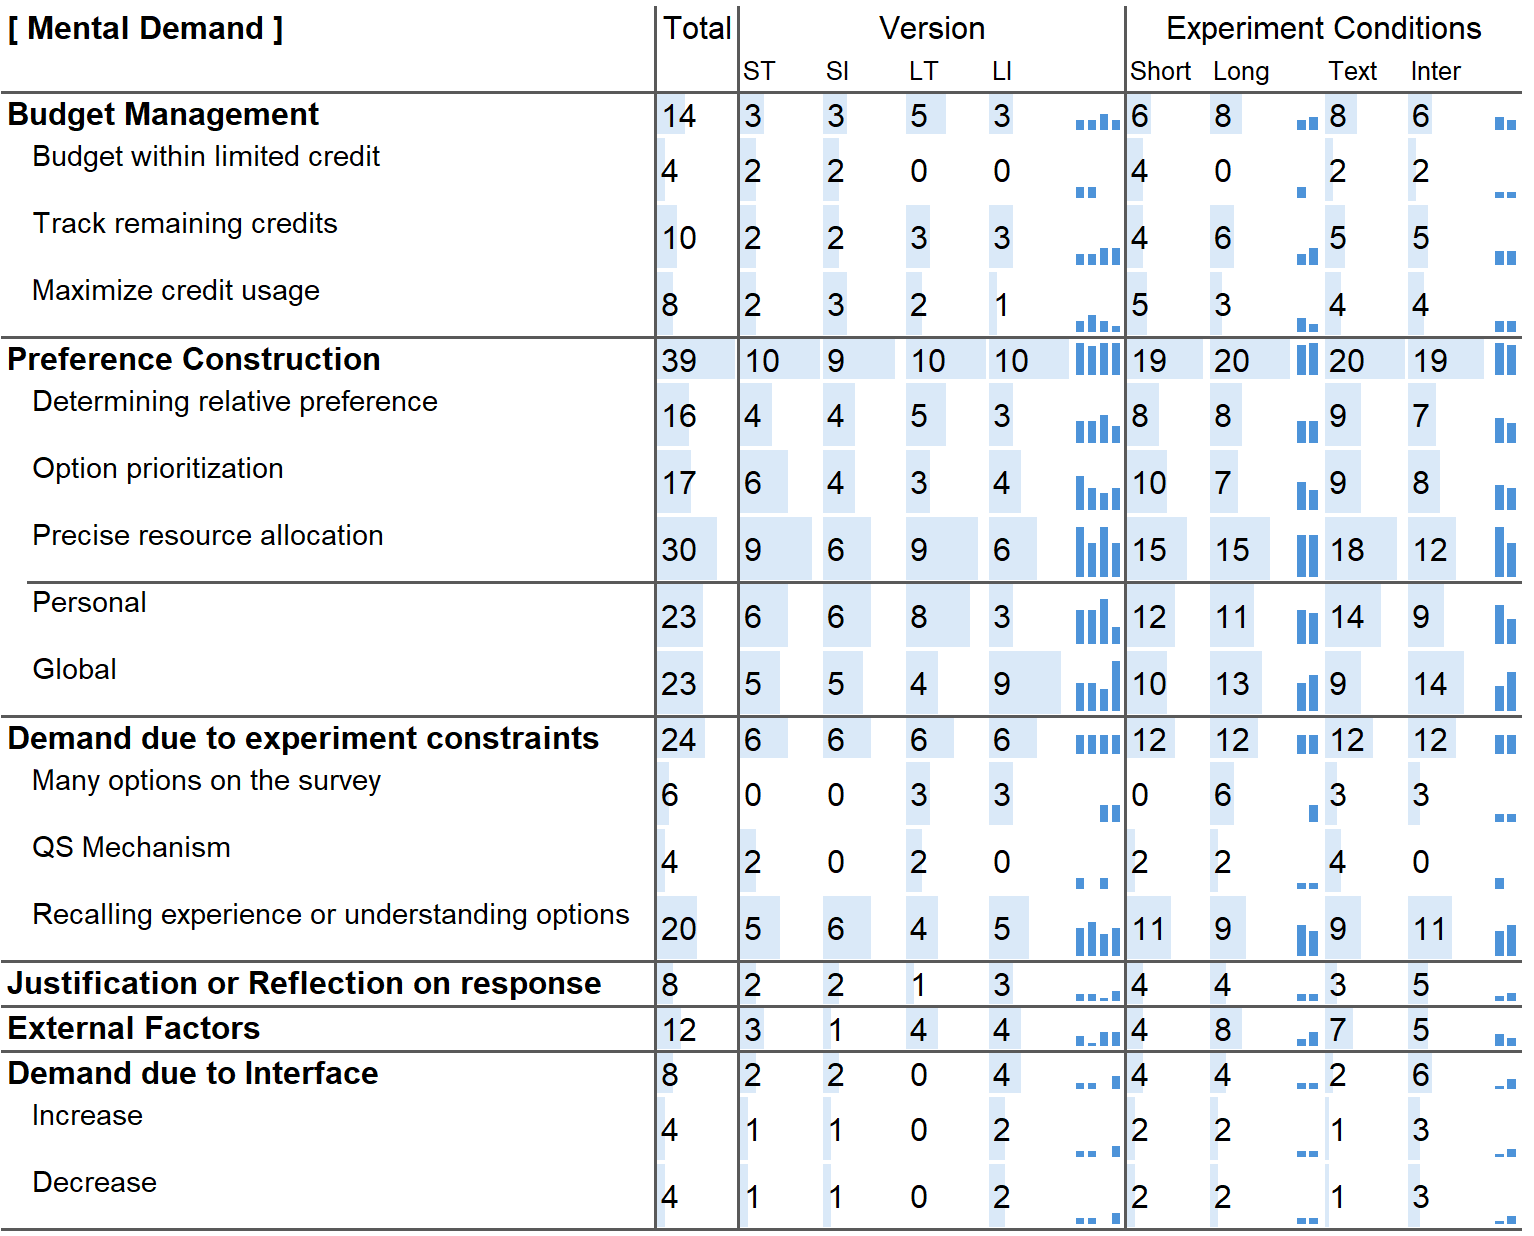
\includegraphics[width=\linewidth]{content/image/cog/mental_table.png}
\end{table}

\begin{figure}[t!]
    \centering
    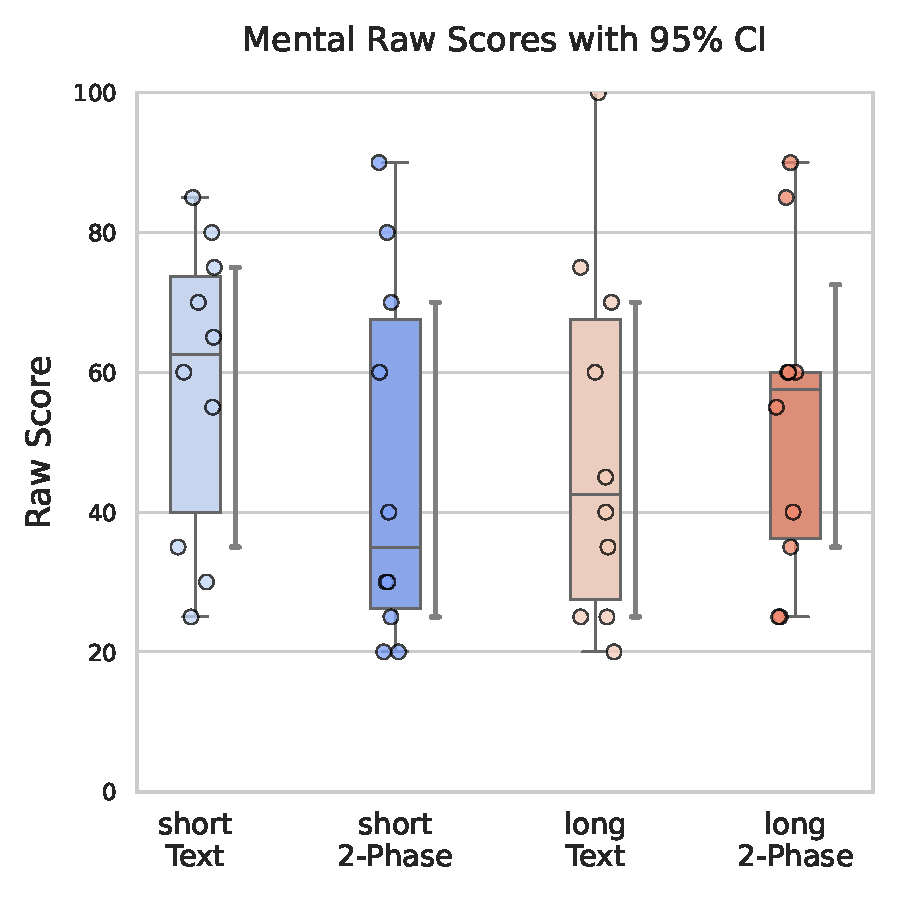
\includegraphics[width=0.48\textwidth, trim=0 13 0 13, clip]{content/image/cog/Mental_scores.pdf}
    \caption{Mental Demand Raw Score: Across all four experiment groups, participants' reported mental demand is spread across a wide range with many participants experiencing high mental demand.}
    \Description{Box plot showing mental raw scores with 95\% confidence intervals across four interface versions: Short Text, Short 2-Phase, Long Text, and Long 2-Phase. The y-axis represents raw scores from 0 to 100. Each box plot includes individual data points. The Short Text and Short 2-Phase versions display wider score distributions, with medians around 60 and 40. The Long Text and Long 2-Phase versions have similar distributions but with slightly lower medians, 40 and 60, respectively. The plot shows a considerable spread in scores, with overlapping confidence intervals, indicating variability in mental demand across all groups.}
    \label{fig:mental_cog_score}
\end{figure}


\subsection{Sources of Physical Demand} 
\label{apdx:physical}
Physical demand refers to the physical effort required to complete a task, such as physical exertion or movement. Most participants reported minimal physical demand~($N=32$), reflected in the low NASA-TLX physical demand scores~(Figure~\ref{apdxfig:physical_cog_score}). Notably, $11$ out of $20$ participants who used the two-phase interface mentioned physical demand from using the mouse, reflecting their increased interaction with the interface. This is further supported by the raw NASA-TLX physical demand scores~(Figure~\ref{apdxfig:physical_cog_score}), which show a significant visual difference between short and long two-phase interfaces as well as between text and two-phase interfaces in long surveys. Table~\ref{apdx:physical_table} presents all the relevant codes across experiment groups.


\begin{table}[h]
    \caption{Physical Demand Causes: Most participants expressed little or no physical demand. Results reflected that participants in the long two-phase interface required more actions, hence the higher mention of mouse usage as a source.}
    \Description{A table showing physical challenges experienced by participants, including Reading, Mouse, Vertical Screen, and None/Little physical effort, with sparklines and percentage bars visualizing the data trends. Data is split across four interface versions (ST, SI, LT, LI) and experiment conditions (Short, Long, Text, Inter). The Mouse category has the highest counts, with trends clearly visible via sparklines and bars, while Reading and Vertical Screen challenges have lower values. The None/Little row shows participants reporting minimal physical effort with percentage bars illustrating the distribution.}
    \label{apdx:physical_table}
    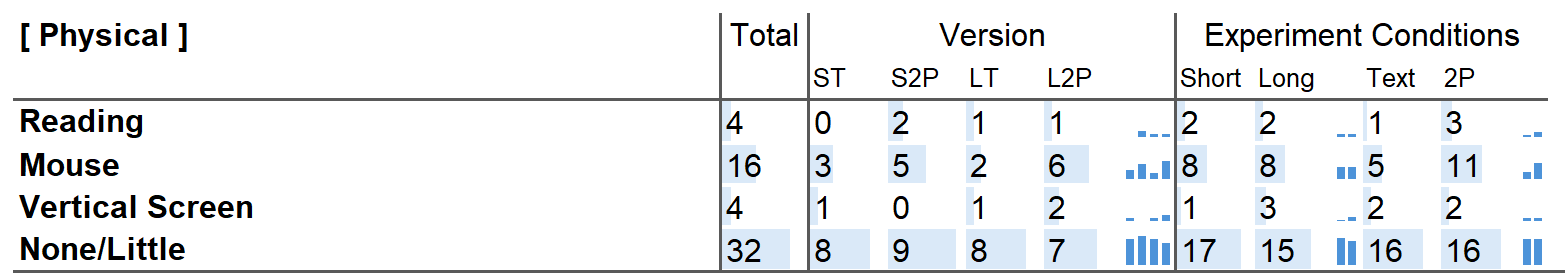
\includegraphics[width=\linewidth]{content/image/cog/physical_table.png}
\end{table}

\begin{figure}[h]
    \begin{minipage}[t]{0.45\textwidth}
        \centering
        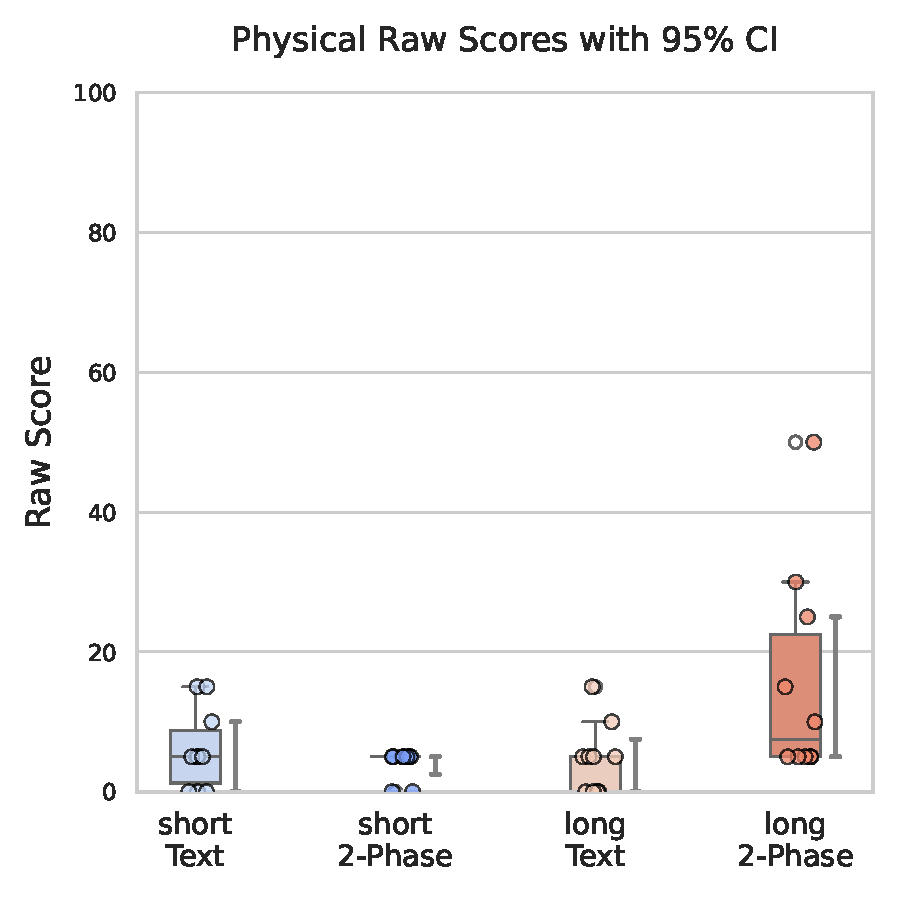
\includegraphics[width=\textwidth, trim=0 13 0 13, clip]{content/image/cog/Physical_scores.pdf}
        \captionsetup{width=0.9\textwidth, justification=justified}
        \caption{Physical Demand Raw Score: Participants other than the long two-phase interface reported minimal physical demand. The long two-phase interface had the highest physical demand, likely due to increased mouse clicks and extended time spent looking at the vertical screen.}
        \Description{A box plot showing the distribution of physical raw scores across four interface versions: Short Text, Short 2-Phase, Long Text, and Long 2-Phase. The y-axis represents the raw score ranging from 0 to 100. The box plots include individual data points, a central line for the median, and whiskers indicating the 95\% confidence interval. The Short Text, Short 2-Phase, and Long Text interfaces show minimal physical demand, with scores clustered below 20. The Long 2-Phase interface exhibits higher physical demand, with a few scores scattered up to around 60.}

        \label{apdxfig:physical_cog_score}
    \end{minipage}
    \hfill
    \begin{minipage}[t]{0.45\textwidth}
        \centering
        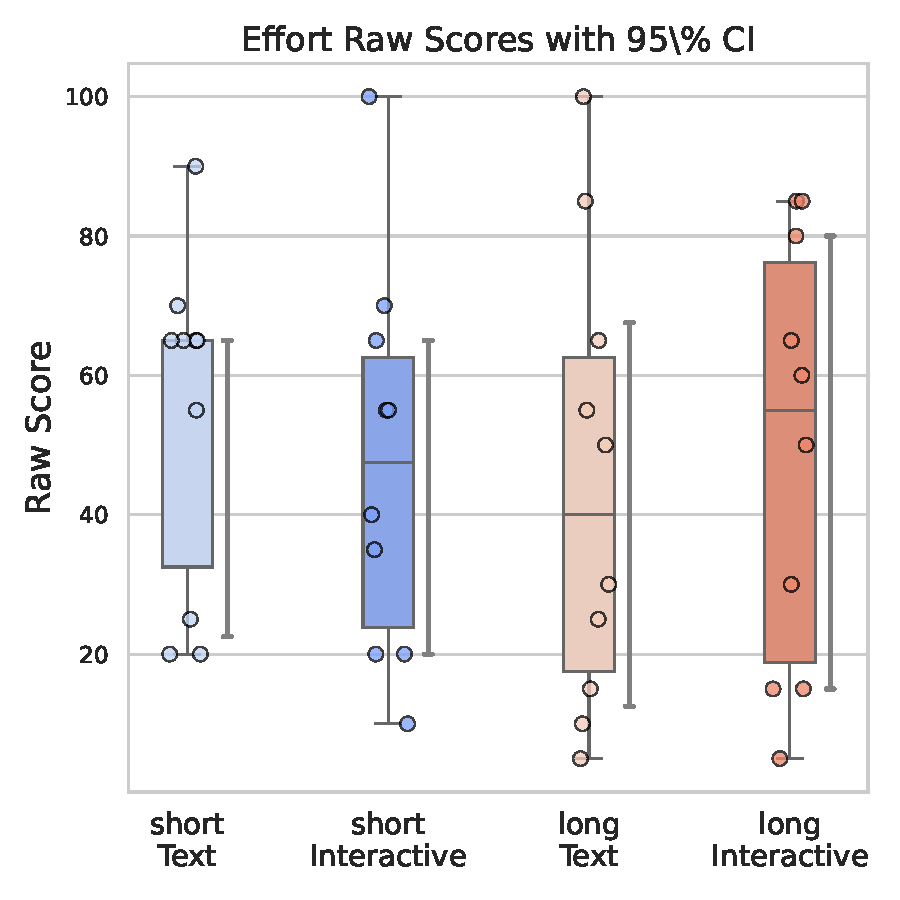
\includegraphics[width=\textwidth, trim=0 13 0 13, clip]{content/image/cog/Effort_scores.pdf}
        \captionsetup{width=0.9\textwidth, justification=justified} % Adjust the width to match the image width
        \caption{Effort Raw Score: Effort scores shows indifference across groups.}
        \Description{A box plot showing the distribution of effort raw scores across four interface versions: Short Text, Short 2-Phase, Long Text, and Long 2-Phase. The y-axis represents the raw score ranging from 0 to 100. Each box plot includes individual data points, a central line indicating the median, and whiskers representing the 95\% confidence interval. The Long 2-Phase interface shows the widest range of effort scores, while the other interfaces display more compact distributions. Data points are scattered within and outside the whiskers, reflecting variability in effort scores across the groups.}
        \label{apdxfig:effort_cog_score}
    \end{minipage}
\end{figure}

% ============================================= %
\begin{table}[h]
    \caption{Effort Sources: Participants using the text interface focused more on operational tasks, while those using the two-phase interface focused more on strategic planning.}
    \Description{A table summarizing participant effort as Operational and Strategic (personal and global), with data visualized using sparklines and percentage bars. The table is split into four versions (ST, SI, LT, LI) and experiment conditions (Short, Long, Text, Inter), with counts and corresponding bars for each category. The operational effort shows participants managing tasks, while the strategic effort captures balancing personal preferences with societal concerns. Sparklines highlight trends across different conditions. A None/Little/A bit row shows participants exerting minimal effort, visualized with bars.}

    \label{apdx:effort_table}
    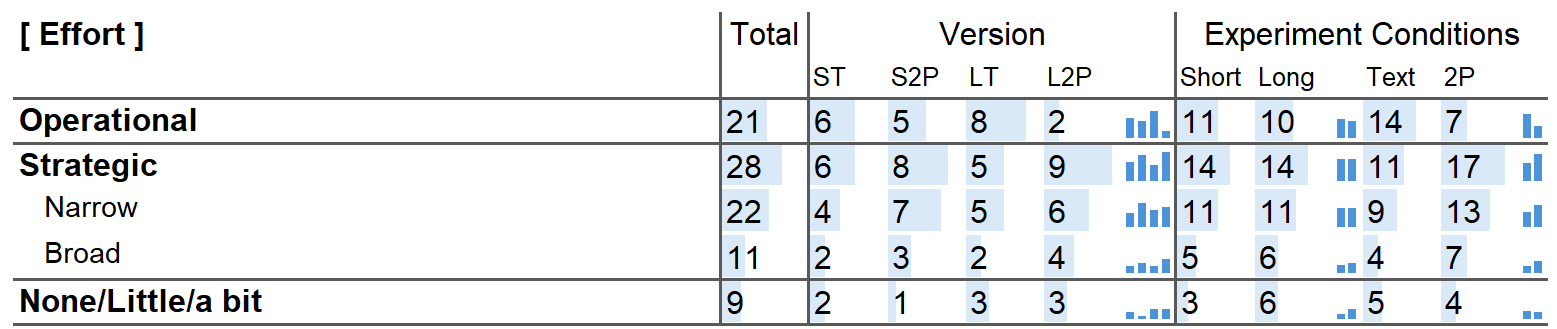
\includegraphics[width=\linewidth]{content/image/cog/effort_table.png}
\end{table}

%\vspace{5pt}
% \begin{tldrbox}
%    \faKey~\textbf{Key Differences:} First, participants in the text interface associated effort with operational tasks more often than participants from the two-phase interface. Conversely, participants in the two-phase interface cited more sources from strategic planning than those in the text interface. We observed that participants experienced effort when considering a comprehensive view while using the two-phase interface.
   
%    %Effort sources varied between operational~\textit{Operational Tasks} and~\textit{Strategic Planning}. Participants using the text interface focused on operational tasks, while those using the two-phase interface engaged in strategic planning. This shows that the two-phase interface spurs deeper, more critical thinking.
% \end{tldrbox}

\subsection{Source of Effort}
\label{apdx:effort}
Effort refers to how hard participants felt they worked to achieve the level of performance they did. Since effort includes both mental and physical resource intensity, refer to \Cref{sec:mental} and \Cref{apdx:physical} for definitions. Raw NASA-TLX effort scores~(Figure~\ref{apdxfig:effort_cog_score}) showed a similar spread across experiment groups, the qualitative analysis showed more distinction that participants using the two-phase interface considered options more comprehensively and felt less effort on completing operational tasks, similar to what we found on mental demands~(Section \ref{sec:mental}). Table~\ref{apdx:effort_table} contains codes.

\subsubsection{Effort Source \#1: Operational Tasks} $14$ of the $20$ participants using the text interface mentioned Operational Tasks as effort sources, compared to $7$ using the two-phase interface, with the lowest mention by the long two-phase interface group~($N=2$). Quotes below illustrated participants putting in effort to manipulate the interface.
\begin{displayquote}
I wanted to bump up~(an option) maybe to 4 or <option> to 5 and realize I couldn't.~\bracketellipsis that would be effort came in of how do I want to really rearrange this to make it~(the budget spending) maximize?

\noindent \hfill -- S029, short text interface
\end{displayquote}
\begin{displayquote}
So it was like it was very~\ldots I have to put a lot of effort in terms of you know~\ldots think about each dimension that if I give one credit to <option name> whether it will affect my credits on <another option name>. \noindent\hfill -- S005, long text interface
\end{displayquote}

\subsubsection{Effort Source \#2: Strategic Planning} Different from Operational Tasks, $11$ participants in the text interface compared to $17$ participants described strategic planning as sources of effort, with almost all participants~($N=9$) from the long two-phase interface. We further categorize strategic planning into \textit{narrow} and \textit{broad} scopes as we did for mental demand~\cref{sec:mental}. Participants using the two-phase interface~($N=7$) had nearly mentioned double~($N=4$) times regarding global strategies. For example:

\begin{displayquote}
And really the bulk of the effort was how to rank order these~(options) and allocate the resources behind the upvotes so that I can accurately depict what I want~\ldots say, a committee to focus on and allocate actual fungible resources, too. \noindent \hfill -- S019, long two-phase interface
\end{displayquote}


% However, qualitative analysis revealed that participants using the text interface experienced more effort focused on operational tasks~(i.e., completing specific tasks). In contrast, participants using the two-phase interface experienced more effort focused on strategic planning~(planning a strategy to complete tasks). Specifically, those using the two-phase interface engaged in global strategic planning, considering options comprehensively and beyond the immediate task. This contrasts with text interface participants, who concentrated more on operational tasks and narrower strategic planning. This finding reinforces that cognitive load sources differ between interfaces, with two-phase interfaces fostering deeper, more critical thinking.

%Both examples show considerations beyond personal experiences, including outcomes or social values. Nearly twice as many participants using the two-phase interface~($N=7$) mentioned global strategic efforts compared to the text interface~($N=4$). Overall, more participants using the two-phase interface~($N=17$) reported sources of strategic effort compared to those using text-based interfaces~($N=11$).

%\subsubsection{Takeaway: Two-phase interface spurs more strategic effort from participants}
%Effort is a realization of mental demand through physical actions. Since participants experienced little physical demand, the sources of effort reflected how individuals translated their mental demand into efforts. The raw NASA-TLX effort scores~(Figure~\ref{fig:effort_cog_score}) showed a similar spread across experiment groups, akin to mental demand. However, qualitative analysis revealed that participants using the text interface experienced more effort focused on operational tasks~(i.e., completing specific tasks). In contrast, participants using the two-phase interface experienced more effort focused on strategic planning~(planning a strategy to complete tasks). Specifically, those using the two-phase interface engaged in global strategic planning, considering options comprehensively and beyond the immediate task. This contrasts with text interface participants, who concentrated more on operational tasks and narrower strategic planning. This finding reinforces that cognitive load sources differ between interfaces, with two-phase interfaces fostering deeper, more critical thinking.

%\begin{wrapfigure}{r}{0.45\textwidth} % Adjust the width as needed
%    \centering
%    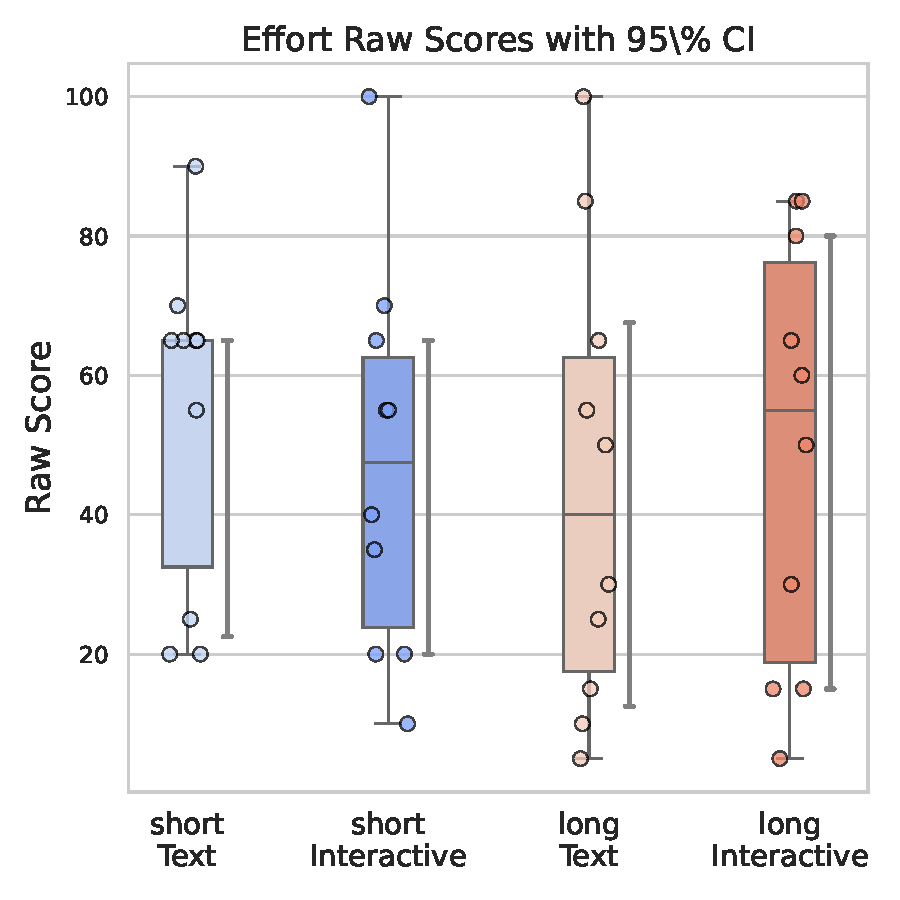
\includegraphics[width=0.45\textwidth, trim=0 13 0 13, clip]{content/image/cog/Effort_scores.pdf}
%    \captionsetup{width=0.40\textwidth, justification=justified} % Adjust the width to match the image width
 %   \caption{Effort Raw Score: Effort scores shows indifference across groups.}
  %  \label{fig:effort_cog_score}
%\end{wrapfigure}


%\subsubsection{Effort Source: Strategic Planning}
%Strategic planning is similar to strategic budget management mentioned under mental demand. Unlike operational tasks, strategic planning involves higher-level strategies to complete the survey. We categorize two distinct types of planning: \textit{personal} and \textit{global}. \textit{Personal strategic planning} involves translating preferences onto the survey without considering broader values or beliefs. For example:

%\begin{displayquote}
%~\bracketellipsis having that prior experience and being able to quickly link it to a tangible thing that I've experienced in my personal life.

%\noindent \hfill -- S032, short text interface
%\end{displayquote}

%\begin{displayquote}
%And really the bulk of the effort was how to rank order these~(options) and allocate the resources behind the upvotes so that I can accurately depict what I want~\ldots say, a committee to focus on and allocate actual fungible resources, too. 

%\noindent \hfill -- S019, long two-phase interface
%\end{displayquote}

%Participants using the two-phase interface~($N=13$) mentioned personal strategic planning slightly more than those using the text interface%\end{displayquote}

%\begin{displayquote}
%Hey, even though I don't really like this idea. But what if they're important? They sort of kind of deserve some attention~\ldots that's why I think I have the effort here.

%\noindent \hfill -- S037, long two-phase interface
%\end{displayquote}
% ============================================= %
\begin{table}[ht]
    \caption{Performance Causes: Most causes are shared across experiment conditions. We provided qualitative interpretations of their own performance assessments.}
    \Description{A table detailing participant performance across Operational Action (budget control, preference reflection, limited resources), Social Responsibility (decision maker, outcome uncertainty), and Performance Assessment (did their best, feel good, good enough). The table includes sparklines and percentage bars to visualize the distribution of performance data across four interface versions (ST, SI, LT, LI) and experiment conditions (Short, Long, Text, Inter). Operational action and social responsibility are visually represented, with sparklines highlighting performance trends.}

    \label{tbl:physical}
    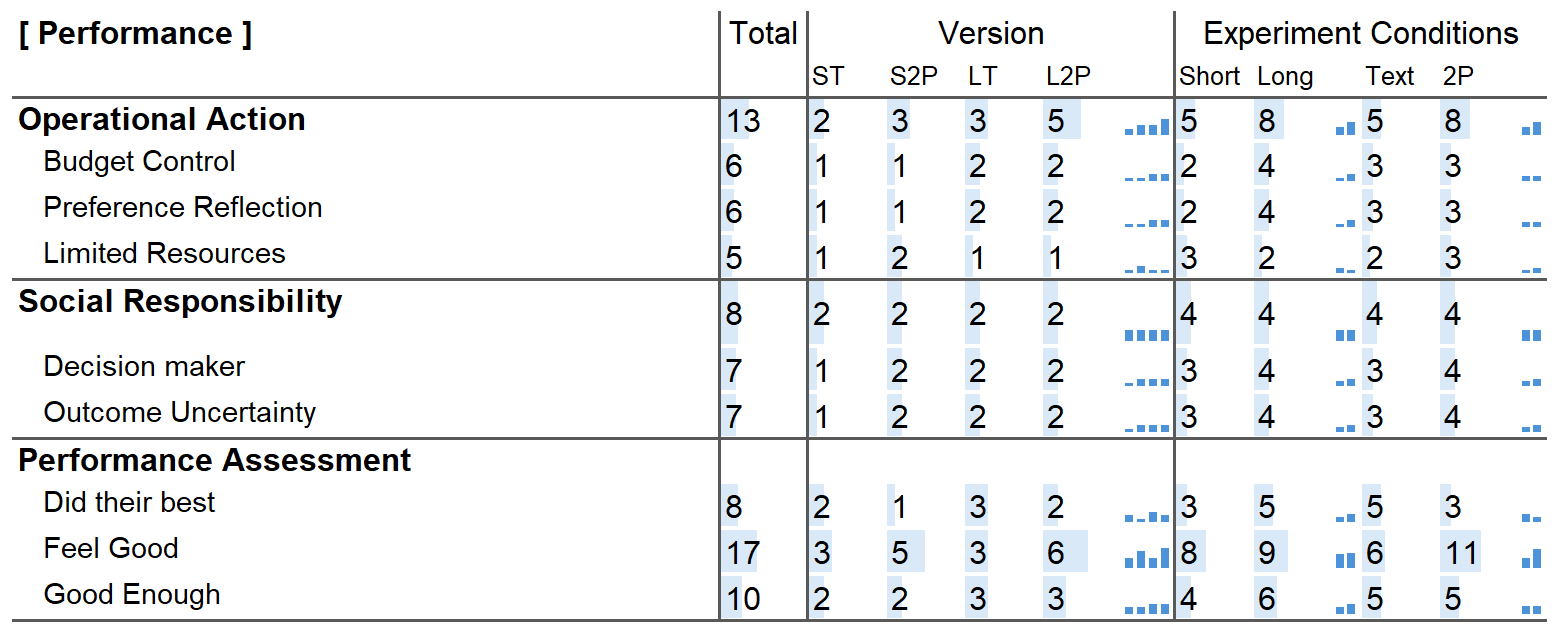
\includegraphics[width=0.95\linewidth]{content/image/cog/perf_table.png}
\end{table}



\begin{figure}[h]
    \begin{minipage}[t]{0.45\textwidth}
        \centering
        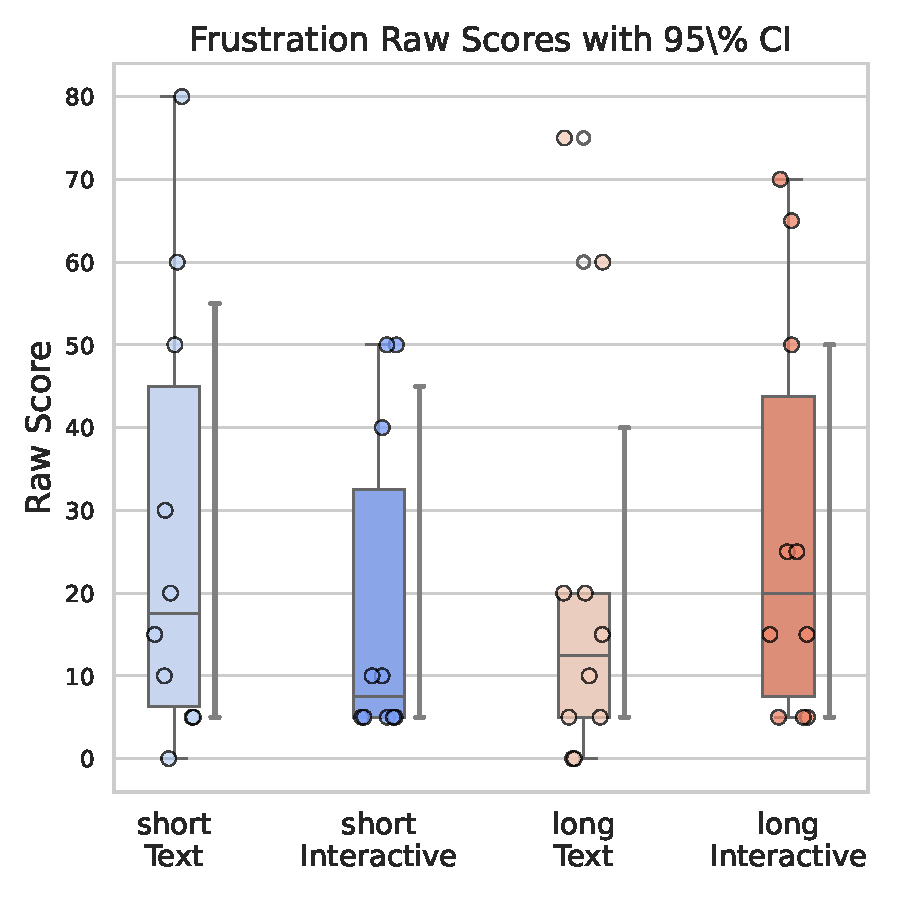
\includegraphics[width=\textwidth, trim=0 13 0 13, clip]{content/image/cog/Frustration_scores.pdf}
        \captionsetup{width=0.9\textwidth, justification=justified}
        \caption{Frustration Raw Score: Participants other than the long text interface highlighted several operational tasks that led to frustration. All groups share causes from strategic planning.}
        \Description{Box plot showing frustration raw scores with 95\% confidence intervals across four interface versions: Short Text, Short 2-Phase, Long Text, and Long 2-Phase. The y-axis represents raw scores from 0 to 100. The Short Text interface has a wide range of scores, with several participants reporting high frustration. The Short 2-Phase interface shows lower median frustration with a narrower distribution. The Long Text interface displays the lowest frustration scores, while the Long 2-Phase interface shows a wide range, with some participants reporting high frustration. Individual data points are included, indicating variability across participants.}
    
        \label{fig:frustration_cog_score}
    \end{minipage}
    \hfill
    \begin{minipage}[t]{0.45\textwidth}
        \centering
        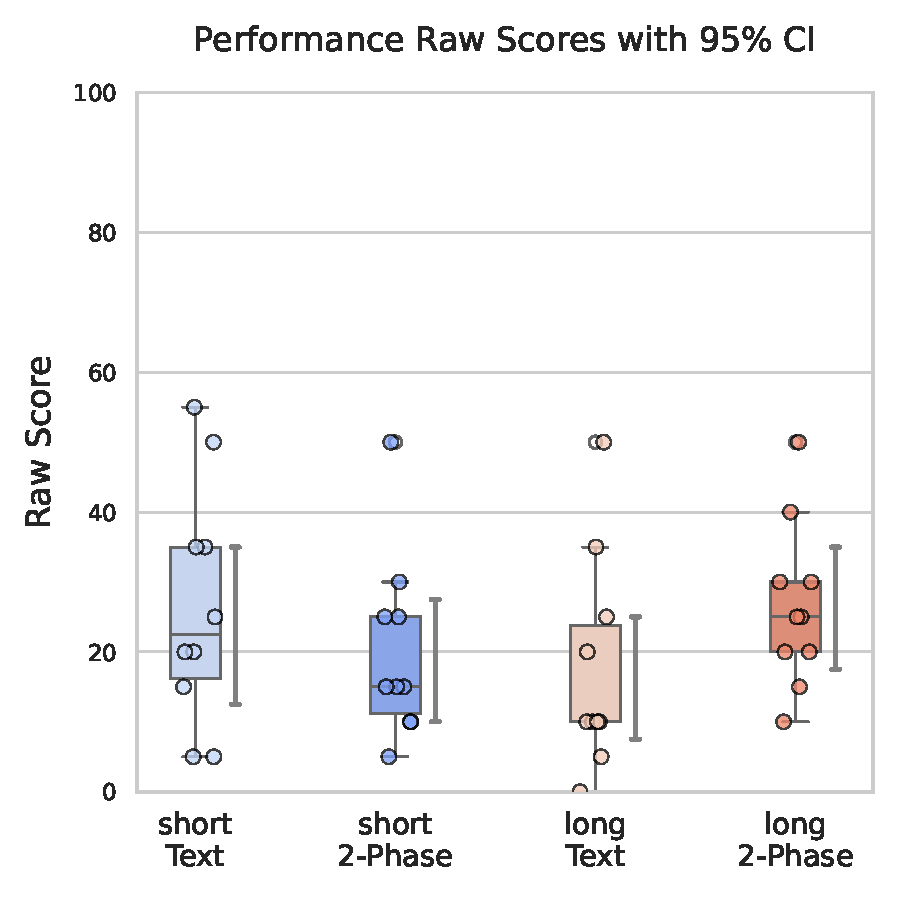
\includegraphics[width=\textwidth, trim=0 13 0 13, clip]{content/image/cog/Performance_scores.pdf}
        \captionsetup{width=0.9\textwidth, justification=justified} % Adjust the width to match the image width
        \caption{Performance Demand Raw Score: Participants showed indifferent performance raw scores across experiment conditions, all trending toward satisfactory.}
        \Description{A box plot displaying the distribution of performance raw scores across four interface versions: Short Text, Short 2-Phase, Long Text, and Long 2-Phase. The y-axis represents raw scores ranging from 0 to 100. Each box plot includes individual data points, a central line for the median, and whiskers representing the 95\% confidence interval. The performance scores appear relatively low across all conditions, with medians hovering between 20 and 40.}
    
        \label{fig:performance_cog_score}
    \end{minipage}
\end{figure}


\subsection{Source from Performance}
\label{apdx:performance}

Performance refers to a person's perception of their success in completing a task. Lower values mean good perceived performance; higher values mean poor perceived performance. We found minimal qualitative differences between experiment groups regarding factors influencing perceived performance. Two influencing factors emerged: \textit{Operational Actions} and \textit{Social Responsibility}. Despite most participants reporting positively on their performance, nuances exist in how different groups interpret their performance.

\subsubsection{Operational Actions}
Operational actions, like the theme presented in temporal demand, refer to specific, executable procedures participants perform in the survey. This could involve: pressure to spend all credits or stay within budget~($N=6$), fears that final vote choices did not reflect true preferences($N=5$), or concerns that they had finished the task inefficiently~($N=6$).


\subsubsection{Social Responsibility}
Social responsibility-based concerns around performance came up when participants reflected on how their final vote counts would be perceived by others~(\smallquote{S041}{I don't want people to think that I just like don't care about <ethnicity> people at all}) or influence real-world decision-making~(\smallquote{S027}{Some of these things might \ldots have outcomes that I didn't foresee}).

All groups cited social responsibility as source to evaluate effort. Raw NASA-TLX scores~(Figure~\ref{fig:performance_cog_score}) show participants had indistinguishable performance scores. This aligns with the interview results where most participants felt positive about their final submission. 

To dig deeper, we also analyzed participants' language when they described their performance. Expressions like ``good enough'' may be indicative of satisficing behaviors -- our results suggest participants are satisfied at similar rates regardless of the interface. 1/4 of the participants in the text interface expressed ``done their best,'' referring to exhausting their effort. Participants who used a two-phase interface were generally more positive about their final outcome -- they were twice as likely to report "feeling good" about their final results~($N=11$ v.s. $N=6$).


\subsection{Temporal Demand}
Table~\ref{apdx:temporal_table} lists all the mental demand codes.
\label{apdx:temporal_table}
\begin{table}[ht]
    \caption{Temporal Demand Sources: Decision-making and Operational Tasks are the main causes. Participants framed their decision-making sources differently.}
    \Description{A table categorizing temporal challenges across Budget Management, Decision Making (affirmative and negative), and Operational (task completion, efficiency). The data includes sparklines and percentage bars to visualize patterns across four versions (ST, SI, LT, LI) and experiment conditions (Short, Long, Text, Inter). Affirmative decision-making shows higher values than negative decision-making, with percentage bars indicating the relative distribution. Temporal operational tasks show consistent effort across conditions, as reflected in the sparklines.}

    \label{tbl:temporal}
    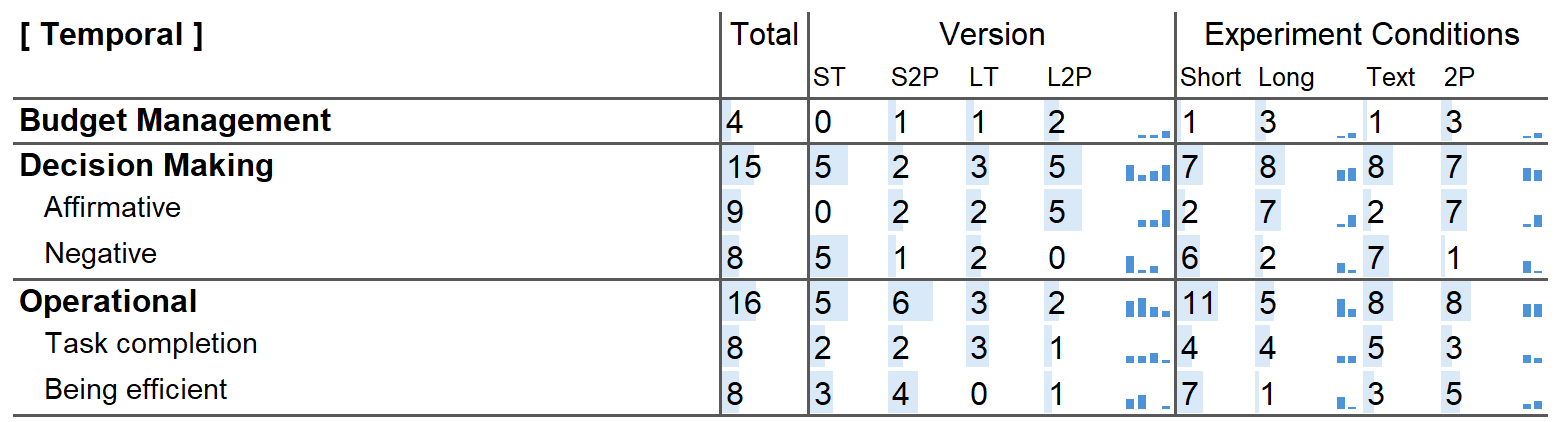
\includegraphics[width=\linewidth]{content/image/cog/temporal_table.png}
\end{table}

\subsection{Frustration}
Table~\ref{apdx:frus_table} lists all the mental demand codes.
\label{apdx:frus_table}
\begin{table}[ht]
    \caption{Frustration Sources: Frustration comes from different levels of strategic operations or operational tasks.}
    \Description{A table with sparklines showing frustration categories: Strategic (higher-level and lower-level) and Operational, across four versions (ST, SI, LT, LI) and experiment conditions (Short, Long, Text, Inter). The table includes sparklines and percentage bars alongside the numerical counts to visually represent the data distribution across conditions. Strategic frustration is divided into higher-level and lower-level conflicts between personal preference and broader societal values. Operational frustration includes challenges such as credit management, adhering to the quadratic mechanism, making decisions, and understanding options. A final row captures participants reporting None/Little frustration, also visualized with percentage bars.}

    \label{tbl:fustration}
    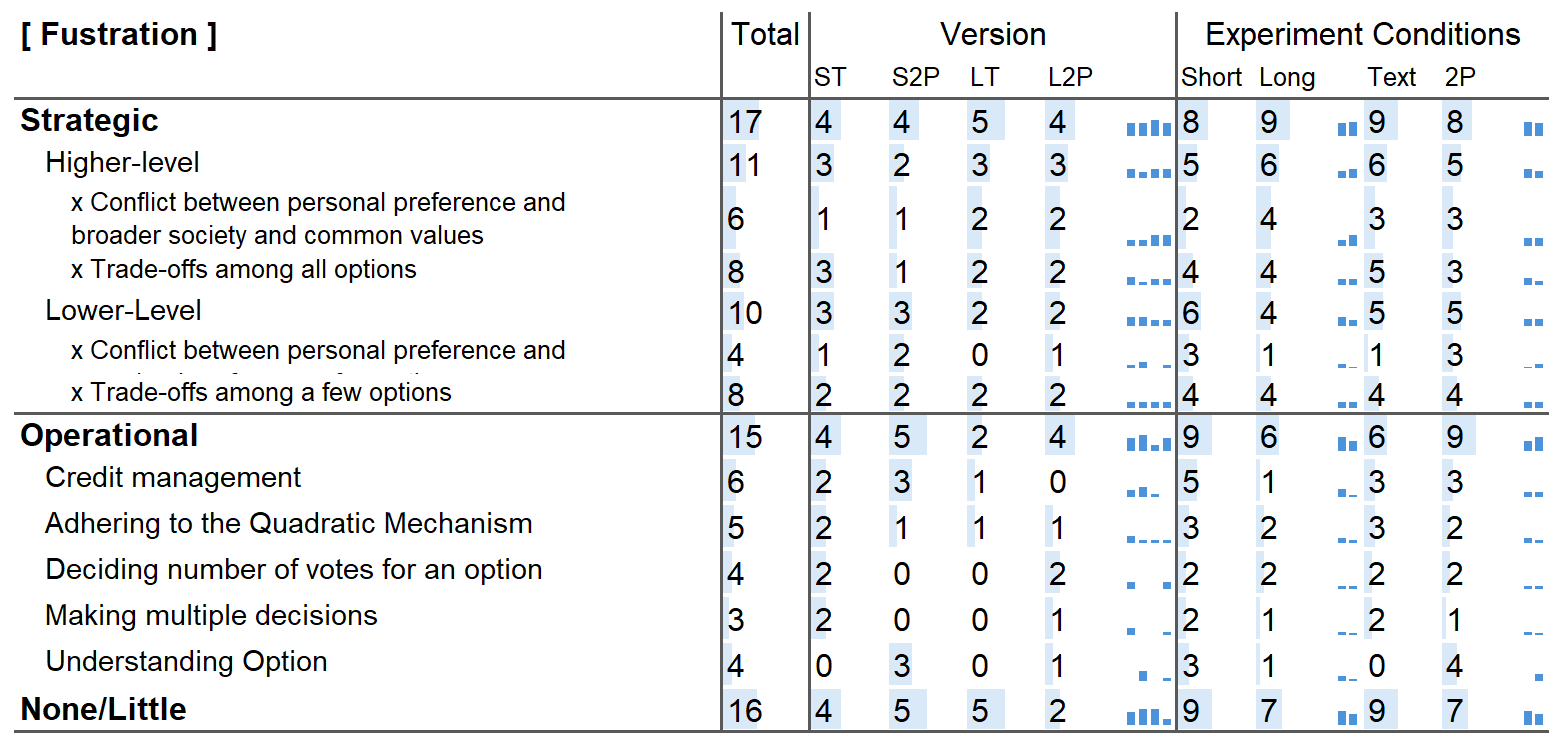
\includegraphics[width=\linewidth]{content/image/cog/fustration_table.png}
\end{table}

% TODO: Need to check the reflective thinking part a bit. I **think** there are differences but it is unclear, need to go back to raw code.

% \begin{figure}[h]
%     \begin{minipage}[t]{0.45\textwidth}
%         \centering
%         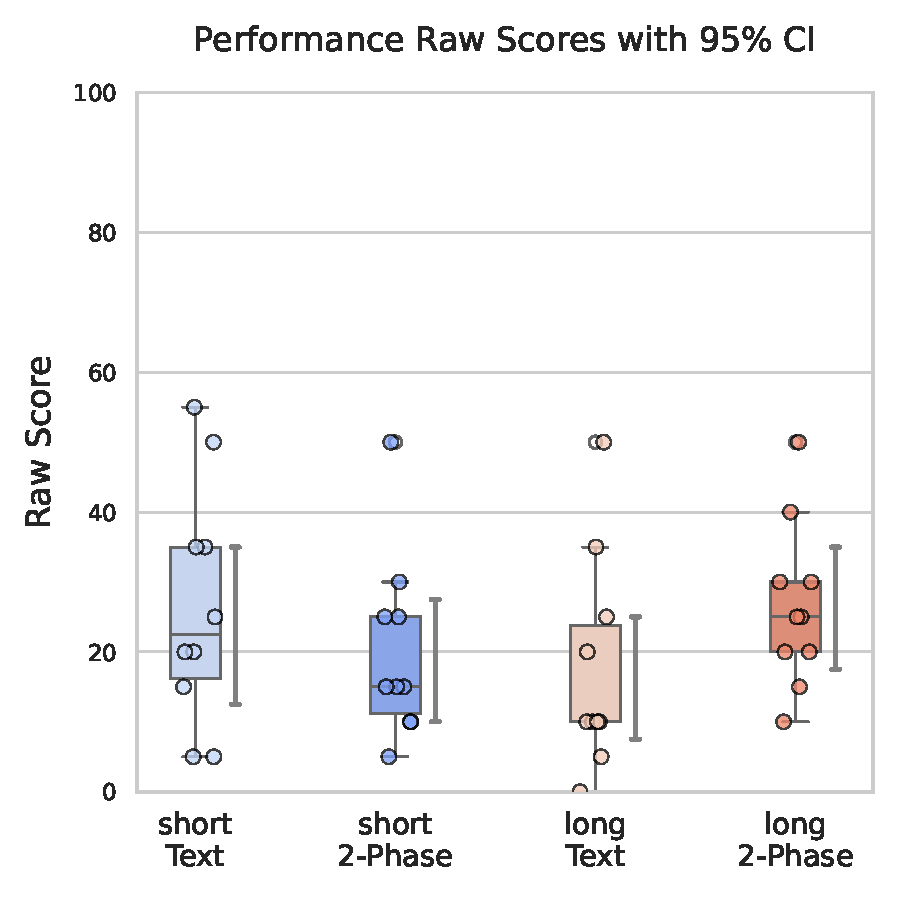
\includegraphics[width=\textwidth, trim=0 13 0 13, clip]{content/image/cog/Performance_scores.pdf}
%         \captionsetup{width=\textwidth, justification=justified} % Adjust the width to match the image width
%         \caption{Performance Demand Raw Score: Participants showed indifferent performance raw scores across experiment conditions, all trending toward satisfactory.}
%         \label{fig:performance_cog_score}
%     \end{minipage}
%     \hfill
%     \begin{minipage}[t]{0.45\textwidth}
%        \centering
%        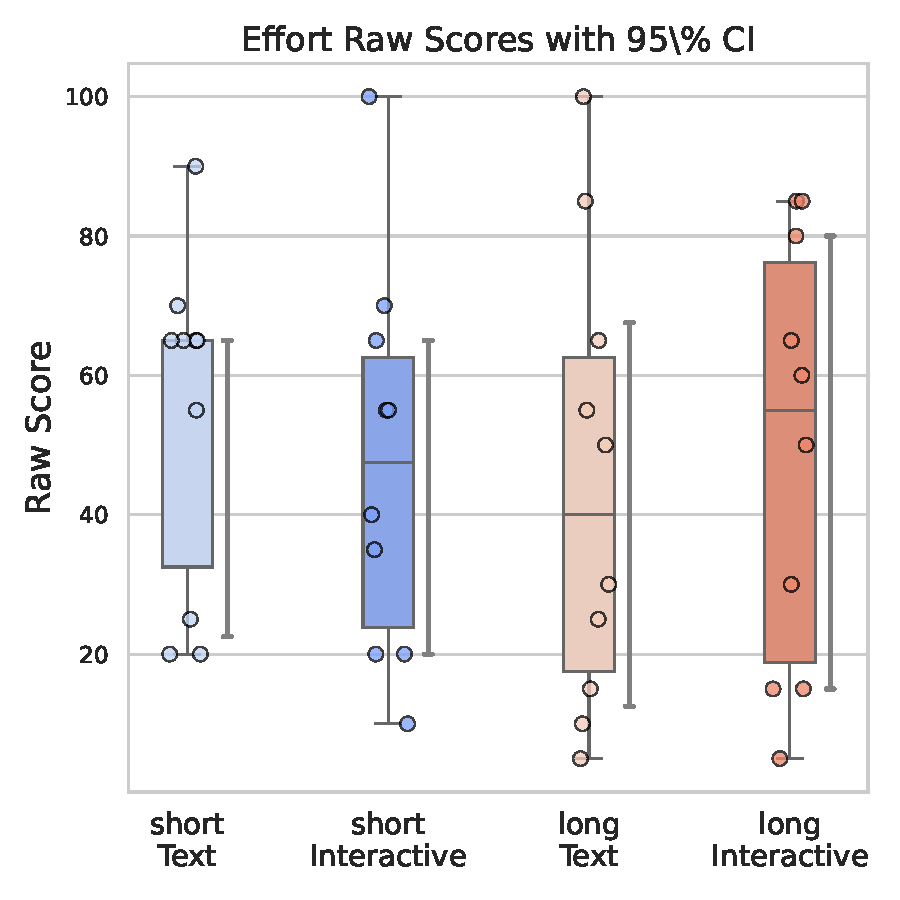
\includegraphics[width=\textwidth, trim=0 13 0 13, clip]{content/image/cog/Effort_scores.pdf}
%        \captionsetup{width=\textwidth, justification=justified} % Adjust the width to match the image width
%        \caption{Effort Raw Score: Effort scores show indifference across groups.}
%        \label{fig:effort_cog_score}
%     \end{minipage}
% \end{figure}